\clearpage
\section{Methods}
\label{sec.methods}

\begin{figure}[!h]
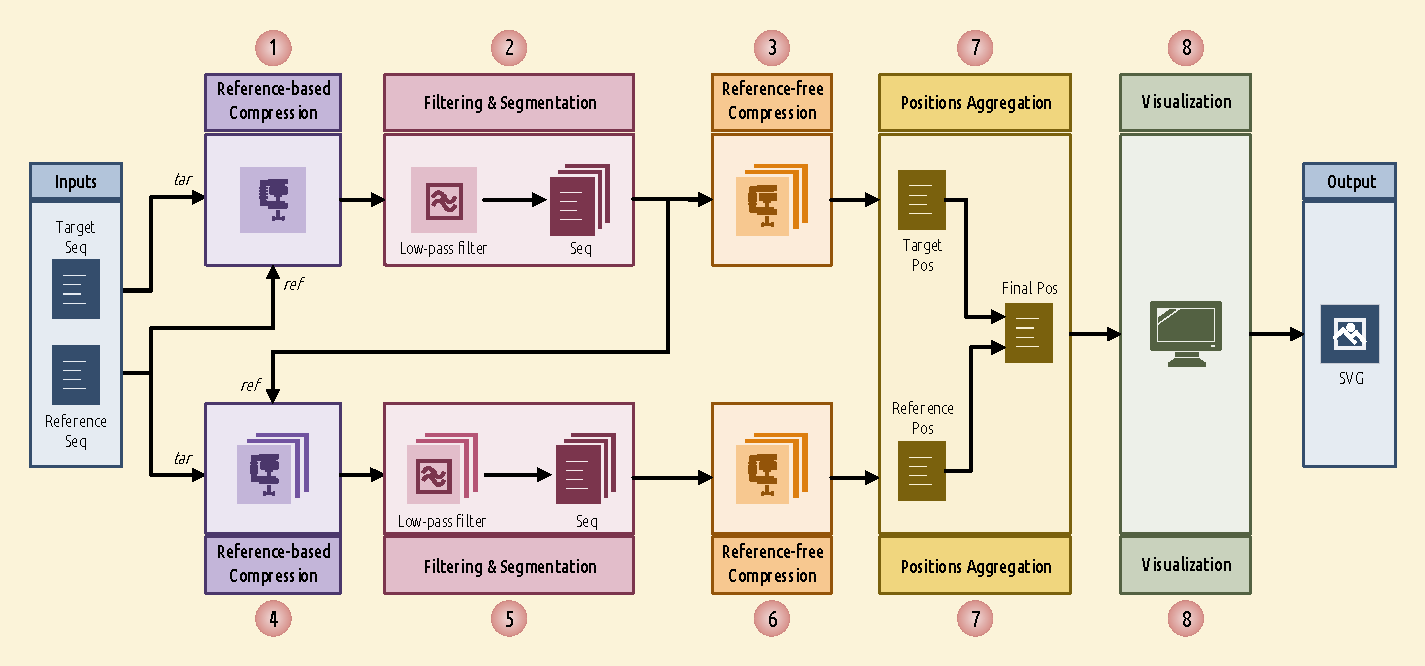
\includegraphics[width=\linewidth]{schema.pdf}
\caption{The schema of Smash++.}
\label{fig.schema}
\end{figure}

\subsection{Building models of the data}

\subsection{finding similar regions}

In order to smooth the profile information, we use Hann window, which is a discrete window function given by
\begin{equation}
  \label{eq.hann}
  w[n]=0.5\;\left[1-\cos \left({\frac {2\pi n}{N}}\right)\right]=\sin ^{2}\left({\frac {\pi n}{N}}\right),
\end{equation}
in which $0\le n\le N$ and length of the window is $N+1$.

\subsection{Computing complexities}

\subsection{The software}

Besides Hann window, that is used as default to filter the profile information obtained by the reference-based compression, we have implemented several other window functions.


% void hamming();
% void hann();
% void blackman();
% void triangular();  // Bartlett window
% void welch();
% void sine();
% void nuttall();